\documentclass[tikz,border=16mm]{standalone}
\usepackage[normalem]{ulem}
\usetikzlibrary{positioning,fit,calc,backgrounds}
\tikzset{block/.style={draw,thick,text width=4cm,minimum height=2cm,align=center},
         line/.style={-latex}
}
\makeatletter
\def\ruwave{\bgroup \markoverwith{\lower7\p@\hbox{\textcolor{red}{\sixly \char116}}}\ULon}
\font\sixly=lasy6
\makeatother


\begin{document}
	\bf
	\LARGE
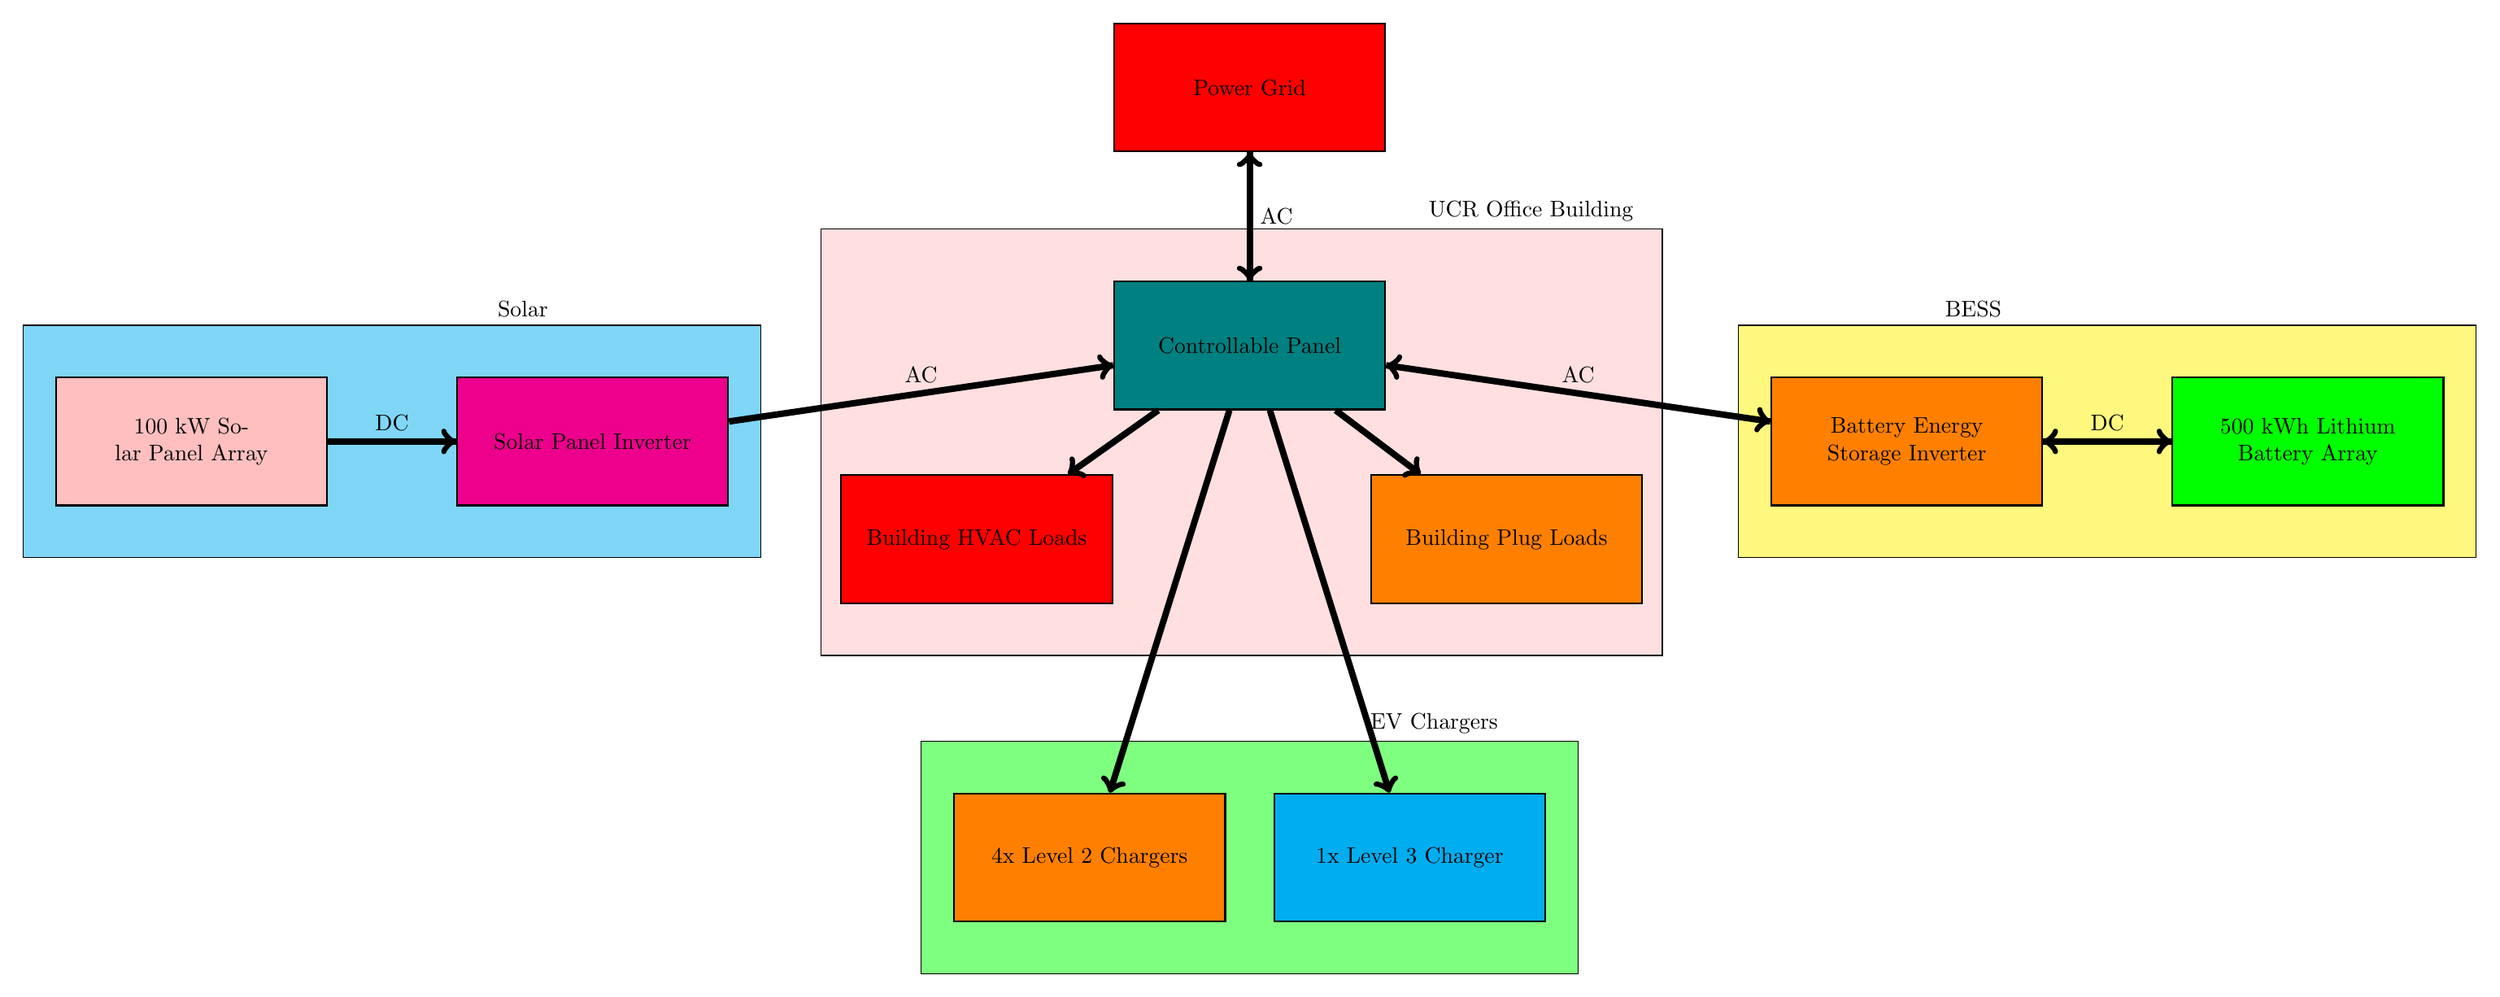
\begin{tikzpicture}
  \node[block, fill = teal] (a) at(0,0) {Controllable Panel};
  \node[block, fill = orange, right=of a, xshift = 5cm, yshift = -1.5cm] (b) {Battery Energy Storage Inverter};
  \node[block, fill = green,right= of b, xshift=1cm] (c) {500 kWh Lithium Battery Array};
  \node[block, fill = magenta, left=of a, xshift  = -5 cm,  yshift = -1.5cm] (d) {Solar Panel Inverter};
  \node[block, fill = pink, left=of d, xshift=-1cm] (e) {100 kW Solar Panel Array};
  \node[block,fill = red, above =of a, yshift = 1cm] (q) {Power Grid};
  \node[block,fill = orange] (l) at (-2.5,-8) {4x Level 2 Chargers};
  \node[block,fill = cyan] (n) at (2.5,-8) {1x Level 3 Charger};
  \node[block,fill=red, below left =of a, xshift = 1cm] (o) {Building HVAC Loads};
  \node[block,fill = orange, below right= of a, xshift = -1.25cm] (j){Building Plug Loads};
%  \node[block,fill = orange, below of= e] (l)  {Level 2 Chargers};
%  \node[block,fill = cyan, below of= q] (n) at {V2G Charger};
  
  
  
  %\node[block] (e) at ([yshift=-2cm]$(b)!0.5!(c)$) {Gate};
  \begin{scope}[on background layer]
   %\node[draw,inner xsep=5mm,inner ysep=6mm,fit=(b)(c),fill=magenta!40]{};
   \node[draw,fill=yellow,fill opacity=0.5,inner xsep=5mm,inner
     ysep=8mm,fit=(b)(c),label={130:BESS}](f){};
  \node[draw,fill=cyan,fill opacity=0.5,inner xsep=5mm,inner
     ysep=8mm,fit=(d)(e),label={50:Solar}]{};
  \node[draw,fill=green,fill opacity=0.5,inner xsep=5mm,inner
  	 ysep=8mm,fit=(l)(n),label={50:\ \ EV Chargers}]{};
  \node[draw,fill=pink,fill opacity=0.5,inner xsep=3mm,inner
	 ysep=8mm,fit=(a)(o)(j),label={50:UCR Office Building}]{};
  \end{scope}
  \draw[<->,line width = 1mm] (q)-- (a) -- node [text width=2.5cm,midway,right,align=left] {AC} (q);
  \draw[<->,line width = 1mm] (a)-- (b) -- node [text width=2.5cm,midway,above,align=center] {AC} (a);
  \draw[<->,line width = 1mm] (b) -- (c) -- node [text width=2.5cm,midway,above,align=center] {DC} (b);
  \draw[->,line width = 1mm] (a) -- (d) -- node [text width=2.5cm,midway,above,align=center] {AC} (a);
  \draw[->,line width = 1mm] (d) -- (e) -- node [text width=2.5cm,midway,above,align=center] {DC} (d);
%  \draw[->,line width = 1mm] (a) -- (l) -- node [text width=2.5cm,midway,above,align=right] {AC} (l);
%  \draw[->,line width = 1mm] (a) -- (n) -- node [text width=2.5cm,midway,above,align=center] {AC} (n);
%  \draw[->,line width = 1mm] (a) -- (o) -- node [text width=3cm,midway,right,align=right] {AC} (o);
%  \draw[->,line width = 1mm] (a) -- (j) -- node [text width=3cm,midway,left,align=left] {AC} (j);
  \draw[->,line width = 1mm] (a) -- (l)  (l);
  \draw[->,line width = 1mm] (a) -- (n)  (n);
  \draw[->,line width = 1mm] (a) -- (o)  (o);
  \draw[->,line width = 1mm] (a) -- (j)  (j);
%  \draw[line] (n) -- (a)  (a);
%  \draw[line] (a) -- (l) -- node [text width=1.0cm,midway,above,align=right] {AC} (l);
%  \draw[line] (a) -- (n) -- node [text width=1.0cm,midway,above,align=right] {AC} (n);
%  \draw[line] (n) -- (a) -- node [text width=1.0cm,midway,above,align=right] {AC} (a);
  
  
  
  %\draw[line] (f.east) -- (c)node[pos=0.4,above]{flow};
  %\draw[line] (e)-- ($(b)!0.5!(c)$);
\end{tikzpicture}
\end{document}